%-----------------begin---preamble-------------------
\documentclass{article}
\usepackage{amsmath,amssymb,amsthm}
\usepackage{tikz,tkz-euclide}
% \usepackage{enumerate}


\usetikzlibrary{calc,patterns,angles,quotes}
\usetkzobj{all}

\def\deg{^{\circ}}
\newcommand\heading[1]{\ \\\large{\textbf{#1}}}
\newcommand\ora[1]{\overrightarrow{#1}}

%------------------end---preamble--------------------

\begin{document}
	\section{Question}
	$ABC$ is an acute angled triangle. The circle with diameter $AB$ intersects the altitude from $C$ at $M$ and $N$. The circle with diameter $AC$ intersects the altitude from $B$ at $P$ and $Q$. Prove $M$, $N$, $P$, and $Q$ all lie on a common circle.
	\section{Solution}
	\begin{figure}[htb!]
	\begin{center}
	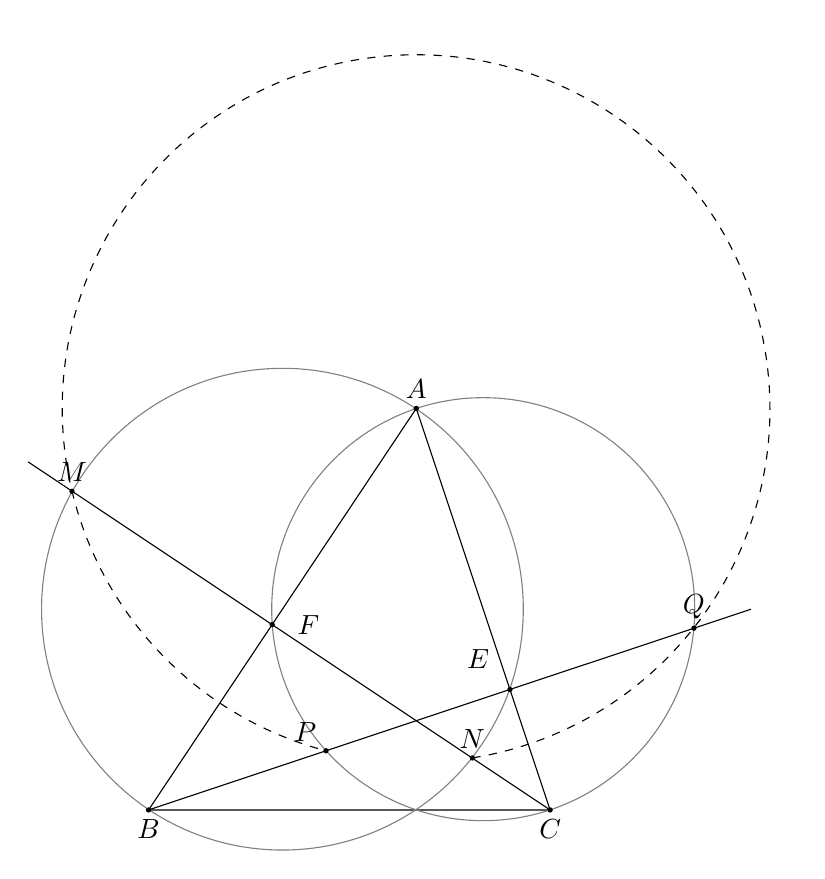
\begin{tikzpicture}[scale=1.7]
		% \useasboundingbox (-2,-2) rectangle  (2,2);
		\coordinate (B) at (-2,-1);
		\coordinate (A) at (0,2);
		\coordinate (C) at (1,-1);
		\tkzDefLine[orthogonal=through C](B,A) \tkzGetPoint{h1};
		\tkzDefLine[orthogonal=through B](C,A) \tkzGetPoint{h2};
		\draw[-] (A)--(B)--(C)--(A);
		\tkzDrawLine[thin,add=0 and 0.3](C,h1);
		\tkzDrawLine[thin,add=1.5 and -1](B,h2);
		\coordinate (m1) at (-1,0.5);
		\coordinate (m2) at (0.5,0.5);
		\tkzDrawCircle[thin](m1,A);
		\tkzDrawCircle[thin](m2,A);
		\tkzInterLC(C,h1)(m1,A)\tkzGetPoints{M}{N};
		\tkzInterLC(B,h2)(m2,A)\tkzGetPoints{P}{Q};
		\tkzInterLL(C,h1)(A,B)\tkzGetPoint{F};
		\tkzInterLL(B,h2)(A,C)\tkzGetPoint{E};
		\node at (A) [above]{$A$};
		\node at (B) [below]{$B$};
		\node at (C) [below]{$C$};
		\node at (E) [above left=0.2]{$E$};
		\node at (F) [right=0.2]{$F$};
		\node at (M) [above]{$M$};
		\node at (N) [above]{$N$};
		\node at (P) [above left]{$P$};
		\node at (Q) [above]{$Q$};
		\tkzDefCircle[circum](M,N,P)\tkzGetPoint{O};
		\tkzDrawArc[thin,dashed](O,N)(P);
		\fill[color=black!100] (A) circle (0.02) ;
		\fill[color=black!100] (B) circle (0.02) ;
		\fill[color=black!100] (C) circle (0.02) ;
		\fill[color=black!100] (E) circle (0.02) ;
		\fill[color=black!100] (F) circle (0.02) ;
		\fill[color=black!100] (M) circle (0.02) ;
		\fill[color=black!100] (N) circle (0.02) ;
		\fill[color=black!100] (P) circle (0.02) ;
		\fill[color=black!100] (Q) circle (0.02) ;
		\end{tikzpicture}
	\end{center}		
	\end{figure}
	Let $E$ and $F$ be the feet of the perpendiculars from $B$ and $C$ respectively.\\
	Note, since $AB$ and $AC$ are diameters. The angles $\angle BNA=\angle CPA=90\deg$. Since we have $\angle NFA=\angle AEP=90\deg$, we get that $AN$ is tangent to the circumcircle of $\triangle NFB$, and $AP$ is tangent to the circumcircle of $\triangle PEC$. Lastly, we know that $BFEC$ is a cyclic quadrilateral. So by using power of a point in the circles $NFB$, $PEC$, and $BFEC$. We get:
	\begin{flalign}
		&&AN^2&=BA \cdot AF= CA \cdot AE =AP^2 &\nonumber \\
		&\therefore& AN&=AP&\nonumber	
	\end{flalign}
	But we already have, $AN=AM$, and $AP=AQ$. Thus,$AN=AM=AP=AQ$. So $M$, $N$, $P$, and $Q$ are all equidistant from $A$, and thus lie on a common circle centred at $A$
\end{document}